\chapter{Physique des particules}\label{ch:b3:particle-physics}

% Provenance (not for print): second half of the "physique subatomique"
% module common to the surveyed third-year curricula: standard model
% inventory, interactions, conservation laws, detectors.

Dépouillez la matière de sa structure, couche après couche ---
molécules, atomes, noyaux, nucléons --- et l'épluchage s'arrête,
brusquement, sur une courte liste~: six \emph{\omterm{def:b3:particle-physics:zoo}{quarks}}, six
\emph{\omterm{def:b3:particle-physics:zoo}{leptons}}, une poignée de porteurs de force, et un scalaire
timide trouvé en 2012. Tout ce que vous avez jamais touché tient en
trois entrées de cette liste~; le reste a vécu dans la première
microseconde de l'univers et revit, brièvement, partout où
$E = mc^2$ est payé rubis sur l'ongle --- collisions de rayons
cosmiques et anneaux d'accélérateurs. Ce chapitre fait l'inventaire~:
les particules, les quatre interactions qui les meuvent, les lois de
conservation (les courants de Noether du
\cref{ch:b3:lagrangian-mechanics}, désormais chargés de la
comptabilité subatomique), et les détecteurs qui photographient le
tout. Il s'achève dans votre propre grenier, à compter des muons
fabriqués dix kilomètres au-dessus.

\section{L'inventaire}

\begin{definition}[Leptons, quarks, hadrons]\label{def:b3:particle-physics:zoo}
\index{lepton}\index{quark}\index{hadron}\index{baryon}\index{méson}\index{antiparticule}
Les briques de la matière sont des fermions de spin $\tfrac12$
(\cref{ch:b3:spin-two-level}, \cref{ch:b3:identical-particles}) en
deux familles de six. Les \emph{leptons} ne sentent pas la force
forte~: l'électron, le muon et le tau (charge $-e$, chacun plus lourd
que le précédent) et leurs trois neutrinos --- presque sans masse,
presque indétectables. Les \emph{quarks} viennent en six saveurs ---
up, down, étrange, charme, beauté, top --- de charges $+\tfrac23e$
(u, c, t) et $-\tfrac13e$ (d, s, b), et on ne les voit jamais seuls~:
le \emph{confinement} les lie en \emph{hadrons} --- des
\emph{baryons} à trois quarks (proton $=$ uud, neutron $=$ udd) et
des \emph{mésons} quark--antiquark (pion, kaon). Chaque particule a
une \emph{antiparticule} de même masse et de charges opposées
(\cref{exo:b3:particle-physics:8}). La matière ordinaire n'emploie
que la première génération --- u, d, e, $\nu_{\text{e}}$~; les deux
copies plus lourdes n'en diffèrent, autant qu'on sache, que par la
masse. «~Qui a commandé cela~?~», demande encore la physique.
\end{definition}

\begin{omfigure}
\begin{tikzpicture}[scale=0.98,
  cell/.style={draw, minimum width=1.28cm, minimum height=1.05cm,
    font=\scriptsize, align=center, inner sep=1pt}]
  % quarks (2x3)
  \foreach \i/\n/\m in {0/u/{$+\tfrac23$}, 1/c/{$+\tfrac23$}, 2/t/{$+\tfrac23$}}
    \node[cell, fill=omDef!18] at (1.4*\i,1.1) {\textbf{\n}\\\m};
  \foreach \i/\n/\m in {0/d/{$-\tfrac13$}, 1/s/{$-\tfrac13$}, 2/b/{$-\tfrac13$}}
    \node[cell, fill=omDef!18] at (1.4*\i,0) {\textbf{\n}\\\m};
  % leptons
  \foreach \i/\n in {0/{e}, 1/{$\mu$}, 2/{$\tau$}}
    \node[cell, fill=omExo!20] at (1.4*\i,-1.35) {\textbf{\n}\\$-1$};
  \foreach \i/\n in {0/{$\nu_{\text{e}}$}, 1/{$\nu_\mu$}, 2/{$\nu_\tau$}}
    \node[cell, fill=omExo!20] at (1.4*\i,-2.45) {\textbf{\n}\\$0$};
  % bosons
  \node[cell, fill=omThm!15] at (5.0,1.1) {\textbf{g}\\forte};
  \node[cell, fill=omThm!15] at (5.0,0) {\textbf{$\gamma$}\\EM};
  \node[cell, fill=omThm!15] at (5.0,-1.35) {\textbf{W, Z}\\faible};
  \node[cell, fill=omThm!15] at (6.5,1.1) {\textbf{H}\\Higgs};
  % generation labels
  \node[font=\scriptsize, anchor=south] at (0,1.75) {1\textsuperscript{re}};
  \node[font=\scriptsize, anchor=south] at (1.4,1.75) {2\textsuperscript{e}};
  \node[font=\scriptsize, anchor=south] at (2.8,1.75) {3\textsuperscript{e}};
  \node[font=\scriptsize, anchor=south] at (5.75,1.75) {médiateurs};
  \node[font=\scriptsize, rotate=90, anchor=south] at (-1.05,0.55) {quarks};
  \node[font=\scriptsize, rotate=90, anchor=south] at (-1.05,-1.9) {leptons};
\end{tikzpicture}

{\small Le tableau du Modèle standard (charges en unités de $e$). Une
seule de ses colonnes bâtit chaque atome~; les deux autres en sont
des échos coûteux. La gravitation, incommensurablement faible à ces
masses, n'a pas de siège à la table --- l'absence la plus célèbre du
modèle.}
\end{omfigure}

\begin{remark}[Quatre interactions]\label{rem:b3:particle-physics:forces}
\index{interaction forte}\index{interaction faible}\index{électrofaible}
Tout processus est l'œuvre de l'une des quatre forces, chacune portée
par son boson. La force \emph{forte} (les gluons) agrippe les \omterm{def:b3:particle-physics:zoo}{quarks}
avec un potentiel qui \emph{croît} avec la distance --- écarter deux
\omterm{def:b3:particle-physics:zoo}{quarks} et le champ étiré claque en une nouvelle paire
quark--antiquark (\cref{exo:b3:particle-physics:1})~: d'où le
confinement, et un résidu de cette force colle les noyaux
(\cref{ch:b3:nuclear-physics}). L'\emph{électromagnétisme} (le
photon, sans masse~: portée infinie) mène la chimie et la lumière. La
force \emph{faible} (W et Z, massifs à
$\approx80$--$\qty{91}{GeV}$~: portée $10^{-3}\,\unit{fm}$, d'où
«~faible~») est la seule à changer la saveur --- la désintégration
$\beta$ est un \omterm{def:b3:particle-physics:zoo}{quark} d devenant un u
(\cref{prop:b3:particle-physics:conservation}) --- et la seule force
à laquelle répondent les neutrinos. La \emph{gravitation} est
$10^{36}$ fois plus faible que l'électromagnétisme entre deux protons
et ne joue aucun rôle de laboratoire --- et pourtant, non écrantée et
de longue portée, elle mènera tout le
\cref{ch:b3:astrophysics}. L'électromagnétisme et la force faible
s'unifient à haute énergie en une seule interaction
\emph{électrofaible} --- séparées, à nos énergies froides, par la
\omterm{def:b3:phase-transitions:order}{brisure de symétrie} du champ de Higgs
(\cref{exo:b3:particle-physics:9}).
\end{remark}

\section{La comptabilité~: les lois de conservation}

\begin{proposition}[Lois de conservation des réactions de particules]\label{prop:b3:particle-physics:conservation}
\index{nombre baryonique}\index{nombre leptonique}\index{lois de conservation!particules}
Une réaction n'a lieu que si les comptes sont justes. Toujours
conservés~: l'énergie--impulsion
(\cref{ch:b3:relativistic-dynamics}), le moment cinétique et la
charge électrique --- le \omterm{thm:b3:lagrangian-mechanics:noether}{théorème de Noether}
(\cref{thm:b3:lagrangian-mechanics:noether}) cautionnant chacun.
Conservés dans toute réaction observée à ce jour~: le \emph{\omterm{prop:b3:particle-physics:conservation}{nombre
baryonique}} $B$ (\omterm{def:b3:particle-physics:zoo}{baryons} $+1$, antibaryons $-1$) et le \emph{\omterm{prop:b3:particle-physics:conservation}{nombre
leptonique}} $L$ (par famille, avec une excellente précision). Ainsi
le proton, le \omterm{def:b3:particle-physics:zoo}{baryon} le plus léger, n'a nulle part où se désintégrer
--- la stabilité de la matière est un théorème de comptabilité ---
et la désintégration $\beta$ doit expédier un antineutrino~:
\[
\text{n} \;\to\; \text{p} + \text{e}^- + \bar\nu_{\text{e}}
\qquad (\text{niveau des quarks~: } \text{d} \to \text{u} +
\text{e}^- + \bar\nu_{\text{e}}) ,
\]
ce qui équilibre $L$ (et explique le spectre continu en énergie de
l'électron, qui a failli coûter à la physique sa foi en la
conservation de l'énergie avant que Pauli n'invente le neutrino pour
la sauver). Les saveurs (étrangeté, charme) sont conservées par les
processus forts et électromagnétiques mais \emph{brisées par le
faible}~: les particules étranges naissent en abondance par paires,
puis meurent lentement et seules --- l'écart de $10^{13}$ entre les
durées de vie fortes de $\qty{e-23}{s}$ et les faibles de
$\qty{e-10}{s}$ est la signature de la force qui a signé la
désintégration.
\end{proposition}
\admitted

\begin{omfigure}
\begin{tikzpicture}[scale=1.0]
  % neutron -> proton beta decay quark diagram
  % three quark lines left to right
  \draw[omDef, thick] (0,2.0) -- (7.2,2.0);
  \draw[omDef, thick] (0,1.45) -- (7.2,1.45);
  \draw[omDef, thick] (0,0.9) -- (3.3,0.9);
  \draw[omThm, thick] (3.3,0.9) -- (7.2,0.9);
  \node[omDef, font=\scriptsize, anchor=east] at (-0.1,2.0) {u};
  \node[omDef, font=\scriptsize, anchor=east] at (-0.1,1.45) {d};
  \node[omDef, font=\scriptsize, anchor=east] at (-0.1,0.9) {d};
  \node[omThm, font=\scriptsize, anchor=west] at (7.3,0.9) {u};
  \node[font=\scriptsize, anchor=west] at (7.3,1.45) {d};
  \node[font=\scriptsize, anchor=west] at (7.3,2.0) {u};
  % W boson wavy-ish (zigzag)
  \draw[omExo, thick] (3.3,0.9)
    -- (3.75,0.55) -- (4.05,0.75) -- (4.35,0.35) -- (4.65,0.55)
    -- (4.95,0.15) -- (5.25,0.35) -- (5.55,-0.05);
  \node[omExo, font=\scriptsize, anchor=west] at (4.75,0.72) {W$^-$};
  % electron and antineutrino
  \draw[thick] (5.55,-0.05) -- (7.2,0.25);
  \draw[thick] (5.55,-0.05) -- (7.2,-0.55);
  \node[font=\scriptsize, anchor=west] at (7.3,0.25) {e$^-$};
  \node[font=\scriptsize, anchor=west] at (7.3,-0.55) {$\bar\nu_{\text{e}}$};
  % braces labels
  \node[font=\scriptsize, anchor=east] at (-0.75,1.45) {neutron};
  \node[font=\scriptsize, anchor=west] at (8.35,1.45) {proton};
\end{tikzpicture}

{\small La désintégration $\beta$, vue au niveau des \omterm{def:b3:particle-physics:zoo}{quarks}~: un
\omterm{def:b3:particle-physics:zoo}{quark} d devient un u en émettant un W$^-$ virtuel, qui se matérialise
en électron plus antineutrino. Tous les comptes tombent juste~: la
charge $-\tfrac13 = +\tfrac23 - 1 + 0$, le \omterm{prop:b3:particle-physics:conservation}{nombre baryonique}, le
\omterm{prop:b3:particle-physics:conservation}{nombre leptonique}.}
\end{omfigure}

\section{Fabriquer et voir des particules}

\begin{remark}[Accélérateurs et détecteurs]\label{rem:b3:particle-physics:machines}
\index{collisionneur}\index{détecteur de particules}
Deux raisons d'accélérer~: la \emph{résolution} --- une sonde ne voit
aucun détail plus fin que sa longueur d'onde $\lambda = h/p$ (le
\cref{ch:b3:crystalline-solids} usait d'ångströms~; les femtomètres
coûtent des \unit{GeV}) --- et la \emph{création}~: l'énergie de
collision devient de la masse nouvelle, et faire entrer en collision
frontale deux faisceaux la dépense tout entière (une cible fixe en
gaspille l'essentiel à emporter les débris vers l'avant~:
\cref{exo:b3:particle-physics:4}). Les collisionneurs circulaires
recyclent les mêmes particules dans le même intervalle accélérateur
pendant que des aimants les guident --- au prix d'un rayonnement
synchrotron $\propto\gamma^4$, et c'est pourquoi l'anneau qui a
trouvé le Higgs fait entrer en collision de lourds protons, non de
légers électrons. Autour du point de croisement s'empilent des
couches en pelure d'oignon, chacune posant une question~: un
\emph{trajectographe} courbe les trajets chargés dans un aimant (la
quantité de mouvement)~; un \emph{calorimètre} électromagnétique
avale électrons et photons (l'énergie)~; un calorimètre hadronique
avale pions et protons~; et seuls les muons percent jusqu'aux
chambres les plus extérieures --- l'identité par la profondeur
d'enfouissement. Les neutrinos partent en impulsion manquante~: la
comptabilité détecte ce que rien ne peut arrêter.
\end{remark}

\begin{omfigure}
\begin{tikzpicture}[scale=1.0]
  % quadrant onion detector
  \fill[omDef!10] (0,0) -- (4.7,0) arc (0:80:4.7) -- cycle;
  \fill[omExo!18] (0,0) -- (3.5,0) arc (0:80:3.5) -- cycle;
  \fill[omThm!12] (0,0) -- (2.3,0) arc (0:80:2.3) -- cycle;
  \fill[white] (0,0) -- (1.2,0) arc (0:80:1.2) -- cycle;
  \foreach \r in {1.2,2.3,3.5,4.7} \draw[gray] (\r,0) arc (0:80:\r);
  \draw[gray] (0,0) -- (4.7,0);
  \draw[gray] (0,0) -- (80:4.7);
  % labels of layers, along the free bottom edge
  \node[font=\tiny, anchor=north] at (1.75,-0.12) {trajectographe};
  \node[font=\tiny, anchor=north] at (2.9,-0.12) {cal.\ é.m.};
  \node[font=\tiny, anchor=north] at (4.1,-0.12) {cal.\ hadr.};
  \node[font=\tiny, anchor=west] at (12:4.85) {chambres à muons};
  % particle tracks from origin
  % electron: curved, stops in ecal
  \draw[omDef, thick] (0,0) .. controls (1.1,0.62) .. (2.05,1.55);
  \fill[omDef] (2.6,1.9) circle (2pt);
  \node[omDef, font=\tiny, anchor=south west] at (2.5,1.98) {e$^-$};
  % photon: straight dashed (neutral), stops in ecal
  \draw[omDef, dashed] (0,0) -- (55:2.75);
  \fill[omDef] (55:2.95) circle (2pt);
  \node[omDef, font=\tiny, anchor=south] at (55:3.2) {$\gamma$};
  % pion: curved into hadronic
  \draw[omThm, thick] (0,0) .. controls (0.75:2.0) and (5:2.6) .. (12:3.9);
  \fill[omThm] (14:4.1) circle (2pt);
  \node[omThm, font=\tiny, anchor=north] at (10:4.28) {$\pi$};
  % muon: nearly straight, exits
  \draw[omExo, very thick] (0,0) .. controls (70:2.4) .. (73:5.2);
  \node[omExo, font=\tiny, anchor=south] at (73:5.35) {$\mu$};
\end{tikzpicture}

{\small Un détecteur de collisionneur en coupe. Chaque espèce écrit
sa signature~: les traces chargées se courbent dans le champ du
trajectographe~; électrons et photons meurent dans le calorimètre
intérieur, les \omterm{def:b3:particle-physics:zoo}{hadrons} dans l'extérieur~; les muons seuls atteignent
les chambres lointaines~; et ce qui s'échappe sans être vu --- le
neutrino --- se lit dans l'impulsion manquante.}
\end{omfigure}

\begin{remark}[Le Higgs, et le grand livre ouvert]\label{rem:b3:particle-physics:higgs}
\index{boson de Higgs}\index{matière noire}
La symétrie du Modèle standard interdit des masses nues à ses
particules~; le \emph{champ de Higgs}, qui emplit tout l'espace d'un
condensat non nul --- le choix du double puits du
\cref{ch:b3:phase-transitions}, promu au rang de vide lui-même ---
brise la symétrie et accorde les masses par ses couplages~: plus la
particule est lourde, plus la prise est ferme. Son propre quantum, le
\omterm{rem:b3:particle-physics:higgs}{boson de Higgs} (\qty{125}{GeV}, trouvé en 2012), a complété le
tableau. Le grand livre ouvert est plus long~: les neutrinos oscillent
entre saveurs et doivent donc avoir une masse que le modèle n'a
jamais inscrite (\cref{exo:b3:particle-physics:10})~; les galaxies
tournent comme si elles étaient tenues par cinq fois plus de matière
qu'il n'en brille (\cref{ch:b3:astrophysics})~; et l'univers contient
de la matière mais presque pas d'antimatière, asymétrie que la
minuscule violation de CP du modèle ne peut pas encore payer. Cette
liste est le programme de ce qui vient ensuite.
\end{remark}

\begin{omfigure}
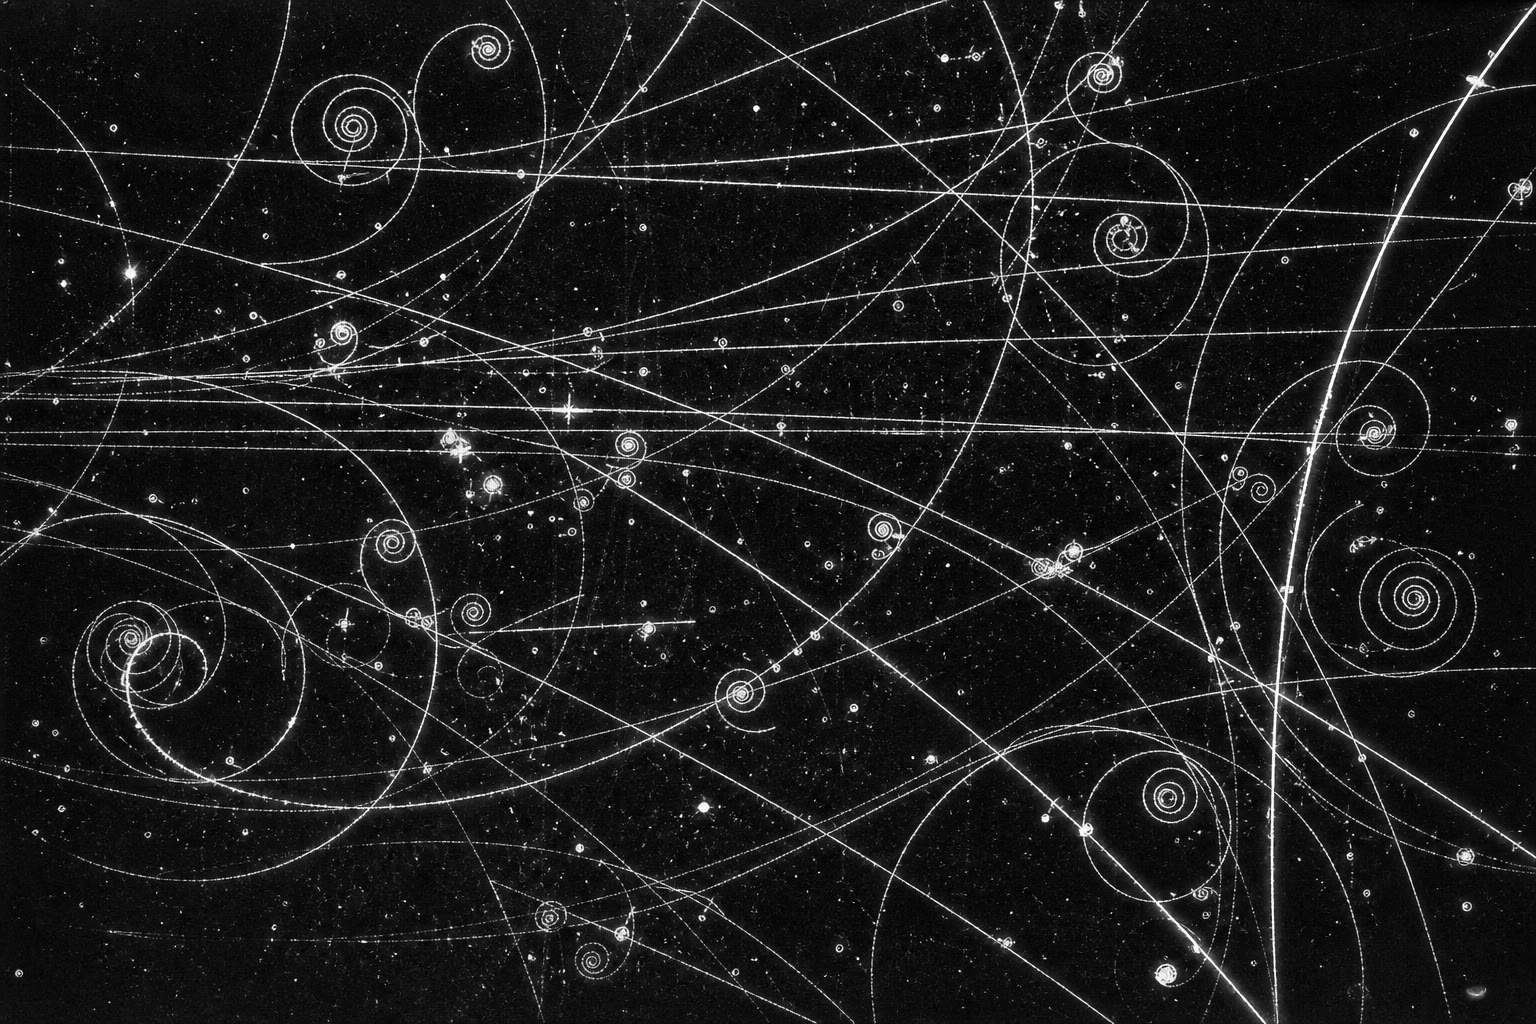
\includegraphics[width=0.58\linewidth]{images/book5/ai/b5-22-bubble-chamber-spirals.jpg}

{\small Une vue de chambre à bulles~: des traces chargées s'enroulant dans un champ magnétique, électrons et positons spiralant en sens contraires à mesure qu'ils perdent leur énergie. Pendant des décennies, la physique des particules s'est lue image par image sur des films comme celui-ci.}
\end{omfigure}

\section{Exercices}

\begin{exercise}[$\star$]\label{exo:b3:particle-physics:1}
Arithmétique des \omterm{def:b3:particle-physics:zoo}{quarks}. (a) Vérifier les charges de p $=$ uud et
n $=$ udd. (b) Le pion $\pi^+$ est $\text{u}\bar{\text{d}}$~:
vérifier sa charge. (c) Proposer un contenu en \omterm{def:b3:particle-physics:zoo}{quarks} pour $\pi^-$ et
pour le $\Delta^{++}$ (charge $+2e$). (d) Pourquoi arracher un \omterm{def:b3:particle-physics:zoo}{quark}
à un proton donne-t-il une gerbe de \omterm{def:b3:particle-physics:zoo}{mésons} plutôt qu'un \omterm{def:b3:particle-physics:zoo}{quark} libre~?
\end{exercise}

\begin{exercise}[$\star$]\label{exo:b3:particle-physics:2}
Trier. Pour chacun de e$^-$, $\nu_\mu$, $\pi^+$, p, n,
$\mu^-$~: (a) \omterm{def:b3:particle-physics:zoo}{lepton}, \omterm{def:b3:particle-physics:zoo}{baryon} ou \omterm{def:b3:particle-physics:zoo}{méson}~? (b) lesquels sentent la force
forte~? (c) lesquels sont stables isolés~? (d) lesquels un champ
magnétique ne peut-il pas dévier~?
\end{exercise}

\begin{exercise}[$\star$]\label{exo:b3:particle-physics:3}
Autorisé ou interdit~? Juger, en nommant la loi violée s'il y en a
une~:
(a) $\text{n} \to \text{p} + \text{e}^- + \bar\nu_{\text{e}}$~;
(b) $\text{p} \to \text{n} + \text{e}^+ + \nu_{\text{e}}$ (pour un
proton \emph{libre})~;
(c) $\text{p} \to \text{e}^+ + \gamma$~;
(d) $\mu^- \to \text{e}^- + \gamma$.
\end{exercise}

\begin{exercise}[$\star$]\label{exo:b3:particle-physics:4}
Le prix de la création. Produire une paire proton--antiproton à
partir d'un faisceau de protons sur une cible d'hydrogène exige (par
l'argument de \omterm{def:b3:relativistic-dynamics:four-momentum}{masse invariante} du
\cref{ch:b3:relativistic-dynamics}) une énergie cinétique de faisceau
de $6m_{\text{p}}c^2$. (a) L'évaluer en GeV. (b) Dans un
collisionneur, deux faisceaux de quelle énergie cinétique suffisent
pour la même paire~? (c) Calculer le rapport de «~gaspillage~» et
expliquer où passe l'énergie en cible fixe. (d) Pourquoi la machine
qui a découvert l'antiproton en 1955 avait-elle besoin de
$\sim\qty{6}{GeV}$~?
\end{exercise}

\begin{exercise}[$\star\star$]\label{exo:b3:particle-physics:5}
Le muon, deux fois. Le muon ($m = \qty{106}{MeV}$,
$\tau = \qty{2.2}{\micro s}$) est le jumeau lourd de l'électron. (a)
Quelle distance représente $c\tau$~? (b) Des muons cosmiques nés à
\qty{15}{km} atteignent le sol~: quel $\gamma$ leur survie
exige-t-elle, et quelle énergie cela fait-il~? (c) Décrire la même
survie dans le référentiel propre du muon. (d) Pourquoi le muon se
désintègre-t-il en un électron mais jamais en un proton, et pourquoi
sa désintégration est-elle \emph{lente} pour les normes des
particules~?
\end{exercise}

\begin{exercise}[$\star\star$]\label{exo:b3:particle-physics:6}
Dans la désintégration $\beta$. (a) Écrire la désintégration du
neutron au niveau des \omterm{def:b3:particle-physics:zoo}{quarks} et vérifier toutes les grandeurs
conservées. (b) Le spectre en énergie de l'électron émis est continu
jusqu'à un point d'arrêt~: expliquer comment cela a jadis menacé la
conservation de l'énergie et comment le neutrino de Pauli l'a sauvée.
(c) Le boson W pèse \qty{80.4}{GeV}~: estimer la portée de la force
faible $\hbar/m_{\text{W}}c$ ($\hbar c = \qty{197}{MeV.fm}$). (d)
Se servir de cette portée pour expliquer en une phrase pourquoi la
force «~faible~» est faible à basse énergie et pourtant aussi forte
que l'électrofaible à haute énergie.
\end{exercise}

\begin{exercise}[$\star\star$]\label{exo:b3:particle-physics:7}
Comptabilité étrange. Les kaons et les hypérons $\Lambda$ portent une
saveur, l'\emph{étrangeté}, conservée par la force forte mais non par
la faible. (a) Expliquer pourquoi les collisions de rayons cosmiques
ne produisent des particules étranges que par paires. (b) Le
$\Lambda$ vit $\qty{2.6e-10}{s}$ --- comparer aux $\qty{e-23}{s}$
des désintégrations fortes et conclure quelle force le tue. (c) Quel
rapport d'échelles de temps sépare les deux, et à quel rapport
quotidien cela se compare-t-il (une seconde contre quoi)~? (d)
Comment ce comportement «~étrange~» --- naissance abondante, mort
réticente --- a-t-il forcé l'invention d'un nouveau nombre
quantique~?
\end{exercise}

\begin{exercise}[$\star\star$]\label{exo:b3:particle-physics:8}
L'antimatière, encaissée. (a) Pourquoi
$\text{e}^+ + \text{e}^- \to \gamma$ (un seul photon) doit-il être
interdit, alors que deux photons conviennent~? (b) Calculer l'énergie
libérée en annihilant un gramme d'antimatière avec un gramme de
matière, et comparer au kilogramme d'uranium fissionné de
\cref{exo:b3:nuclear-physics:9}. (c) Les scanners TEP
(\cref{exo:b3:nuclear-physics:12}) fonctionnent aux positons~: d'où
viennent les positons de la médecine~? (d) Fabriquer des antiprotons
coûte $\sim10^{6}$ fois leur \omterm{def:b3:relativistic-dynamics:momentum-energy}{énergie de masse} en puissance prise à la
prise~: commenter l'antimatière comme carburant.
\end{exercise}

\begin{exercise}[$\star\star\star$]\label{exo:b3:particle-physics:9}
Le Higgs comme \omterm{def:b3:phase-transitions:order}{transition de phase}. (a) Reformuler, dans le langage
de \cref{exo:b3:phase-transitions:12}, ce que signifie que le vide
siège dans un puits à symétrie brisée. (b) Pourquoi les W et Z
acquièrent-ils une masse tandis que le photon reste sans masse
(quelle part de la symétrie survit)~? (c) Le \omterm{rem:b3:particle-physics:higgs}{boson de Higgs} est
l'oscillation radiale du champ~: qu'est-ce qui joue ce rôle dans
l'aimant de \cref{thm:b3:phase-transitions:meanfield}~? (d) Au-dessus
de $\sim10^{15}\,\unit{K}$ la symétrie se rétablit~: où et quand
l'univers a-t-il été si chaud pour la dernière fois
(\cref{ch:b3:astrophysics})~?
\end{exercise}

\begin{exercise}[$\star\star\star$]\label{exo:b3:particle-physics:10}
Des neutrinos par milliards. (a) Le Soleil fait deux neutrinos par
cycle $4\text{p} \to {}^4\text{He}$ (\qty{26.7}{MeV})~: à partir de
la constante solaire \qty{1360}{W/m^2}, calculer le flux de neutrinos
à la Terre. (b) Combien traversent votre ongle
(\qty{1}{cm^2}) par seconde, et combien environ interagiront avec
votre corps en une vie (prendre comme donnée une probabilité
d'interaction de l'ordre de $10^{-22}$ par mètre de chair et par
neutrino)~? (c) Les premiers
détecteurs n'attrapaient qu'un tiers des $\nu_{\text{e}}$ prédits~:
énoncer la résolution (les oscillations) et sa conséquence
structurelle pour le Modèle standard. (d) Pourquoi un détecteur de
neutrinos vit-il sous une montagne~?
\end{exercise}

\begin{exercise}[$\star\star\star$]\label{exo:b3:particle-physics:11}
Chiffres de machine. Protons du LHC~: $E = \qty{6.8}{TeV}$ chacun.
(a) Calculer $\gamma$ et $1 - v/c \approx 1/2\gamma^2$. (b) Quelle
longueur d'onde $\lambda \approx hc/E$ sonde la structure, et
comparer au rayon de \qty{0.8}{fm} du proton. (c) Énergie de
collision frontale~: \qty{13.6}{TeV} --- combien de masses au repos
de proton cela pourrait-il créer~? (d) La perte synchrotron varie
comme $\gamma^4$~: calculer le rapport des $\gamma$ électron sur
proton à énergie fixée et justifier les protons pour l'anneau, les
électrons pour les machines de précision.
\end{exercise}

\begin{exercise}[$\star\star\star$]\label{exo:b3:particle-physics:12}
Messagers du bout du monde. Le rayon cosmique le plus énergétique
jamais enregistré portait $\sim\qty{3e20}{eV}$ --- un unique proton.
(a) Convertir en joules et nommer un objet macroscopique doté de
cette énergie cinétique. (b) Calculer son $\gamma$, et la largeur de
la Galaxie ($\sim10^{5}$ années-lumière) dans son propre
référentiel. (c) Au-dessus de $\sim\qty{5e19}{eV}$, les protons
diffusent sur le fond diffus cosmologique
(\cref{ch:b3:photons-phonons}) --- expliquer qualitativement pourquoi
l'univers leur est opaque. (d) Pourquoi de telles énergies, bien
au-delà de tout accélérateur, nous enseignent-elles tout de même
moins que le LHC~? (Penser au flux et au contrôle.)
\end{exercise}

\begin{omfigure}
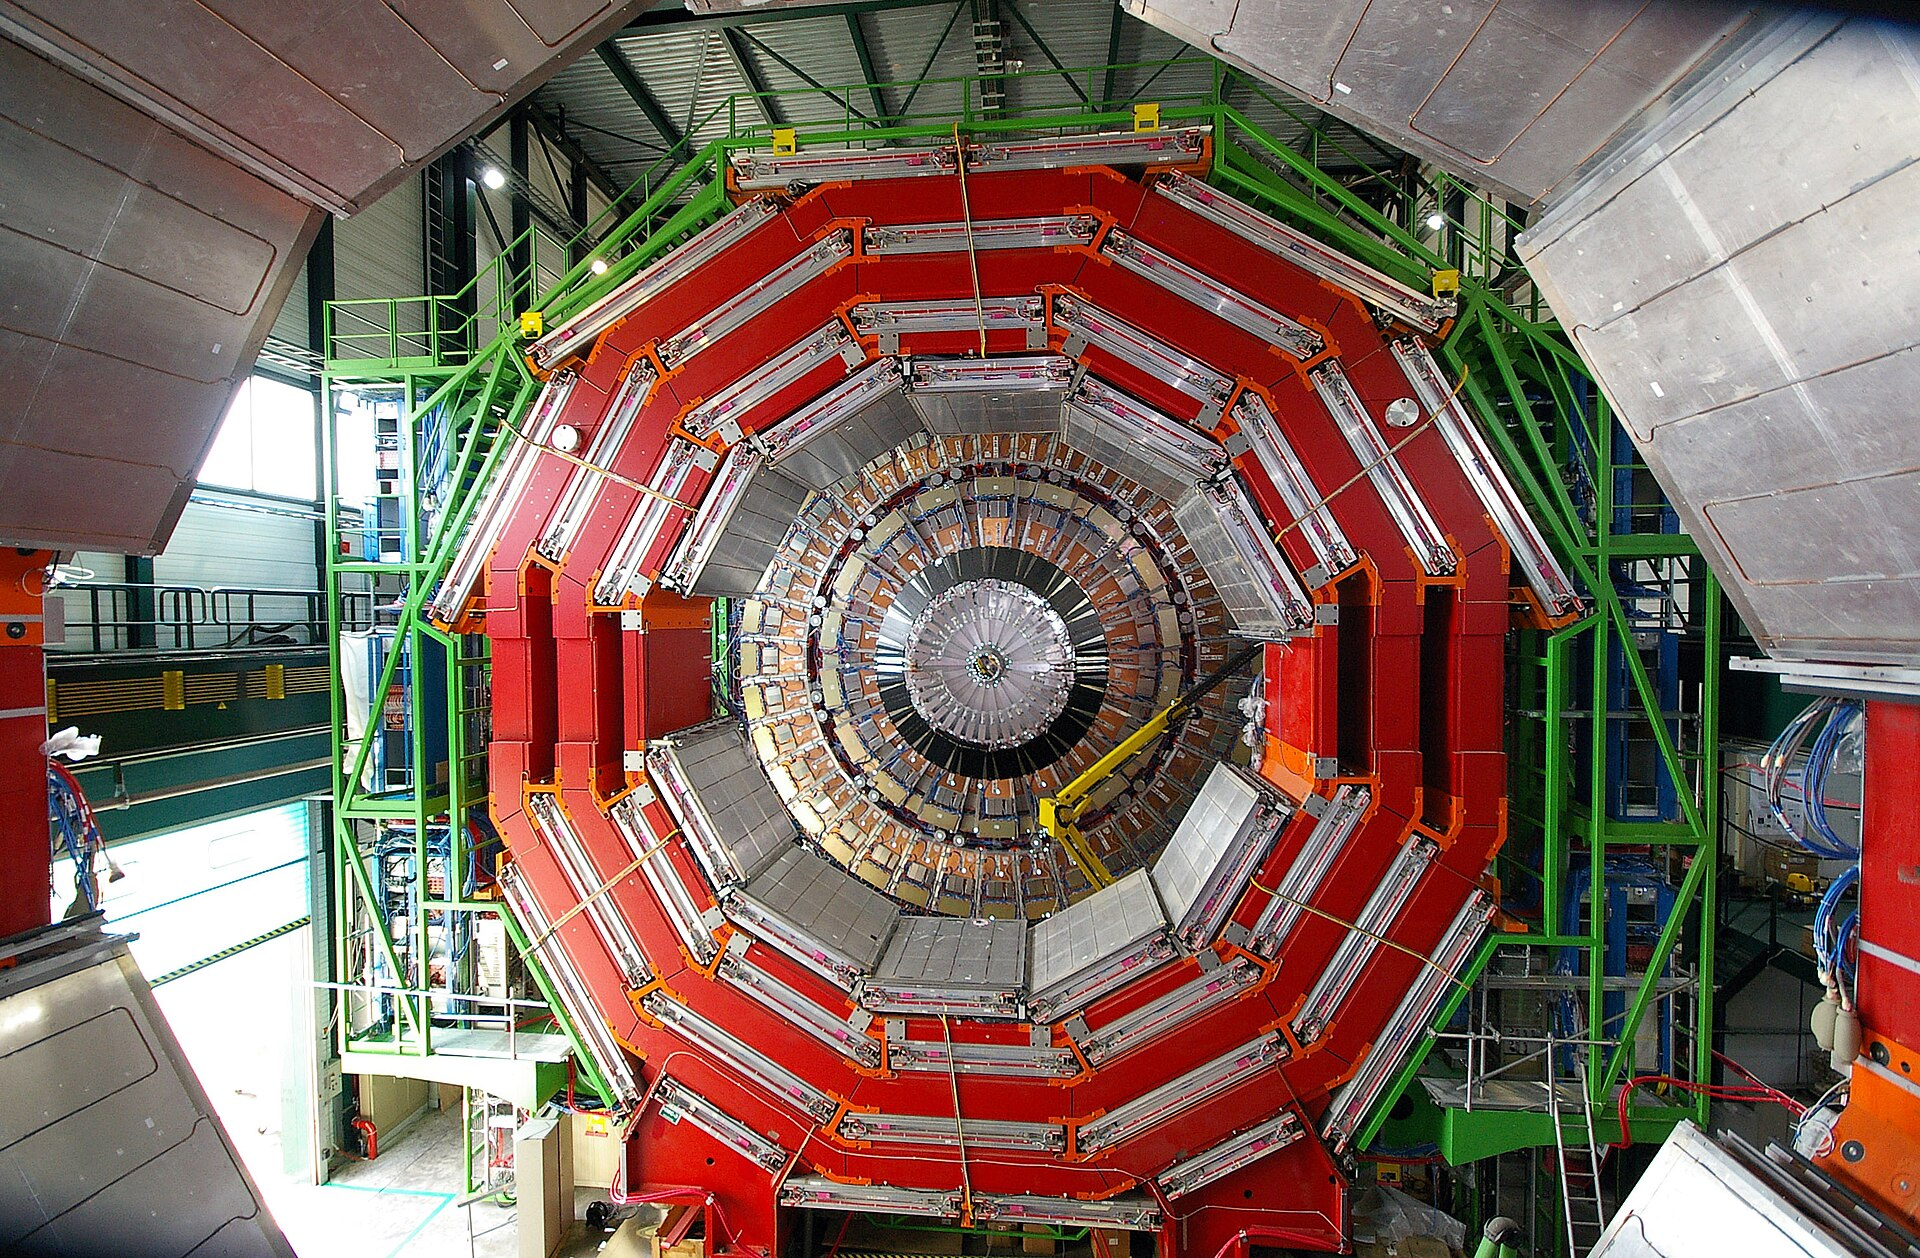
\includegraphics[width=0.62\linewidth]{images/book5/photo-cms-construction.jpg}

{\small Le détecteur CMS en construction (photographie~: Julian Williams, libre d'usage)~: les couches en pelure d'oignon du tonneau, vues de face, avant fermeture --- une réalisation de quinze mille tonnes de la dernière figure de ce chapitre.}
\end{omfigure}

\section{Problème~: le télescope à muons du grenier}

\begin{problem}\label{pb:b3:particle-physics:1}
\emph{Le télescope à muons du grenier.} Pour la fête de la science
vous construisez un télescope à rayons cosmiques~: deux palettes de
scintillateur de $20\times20$\,\unit{cm}, l'une \qty{30}{cm} au-dessus
de l'autre, chacune lue par un photomultiplicateur, câblées en
coïncidence --- un comptage seulement quand les \emph{deux} se
déclenchent en moins de \qty{100}{ns}. Flux de muons au niveau de la
mer à travers une surface horizontale~: environ 1 par \unit{cm^2} et
par minute.

\medskip\noindent\textbf{Partie I --- Compter le ciel.}

\begin{enumerate}
  \item D'où partent vos muons~? Retracer la chaîne~: proton
        primaire, haute atmosphère, pions, muons --- en nommant
        quelle force régit chaque étape.
  \item Pourquoi les pions eux-mêmes n'atteignent-ils presque
        jamais le sol ($\tau_\pi = \qty{26}{ns}$), tandis que leurs
        filles les muons y parviennent~?
  \item Prédiser le taux d'une palette seule à partir du flux
        annoncé.
  \item La palette seule clique en réalité bien plus souvent ---
        bruit électronique et radioactivité ambiante
        (\cref{ch:b3:nuclear-physics}). Expliquer comment la
        coïncidence à deux palettes en supprime la quasi-totalité.
  \item Quel taux de coïncidences fortuites deux sources de bruit
        indépendantes de \qty{100}{Hz} produisent-elles dans une
        fenêtre de \qty{100}{ns} ($R_{\text{acc}} = R_1R_2\Delta t$)~?
        Comparer au vrai taux de muons.
  \item Votre taux de coïncidence se stabilise vers 100 par minute
        --- bien au-dessous des 400 d'une palette seule.
        Expliquer~: quels muons la géométrie à deux palettes
        accepte-t-elle~?
  \item Incliner le télescope~: le taux tombe à peu près comme
        $\cos^2\theta$ de l'angle zénithal. Donner la raison
        physique (qu'est-ce qui croît avec $\theta$~?).
\end{enumerate}

\medskip\noindent\textbf{Partie II --- La relativité, vérifiée au grenier.}

\begin{enumerate}[resume]
  \item Les muons~: $\tau = \qty{2.2}{\micro s}$. Calculer $c\tau$
        et conclure ce que pourrait faire un muon \emph{classique}
        né à \qty{15}{km}.
  \item Vos muons ont en moyenne $E \approx \qty{4}{GeV}$
        ($m_\mu c^2 = \qty{106}{MeV}$)~: calculer $\gamma$.
  \item Durée de vie dilatée, et portée correspondante~: le taux
        du grenier a-t-il maintenant du sens~?
  \item Raconter la survie depuis le référentiel du muon
        (\cref{ch:b3:relativistic-kinematics}).
  \item Pour $\gamma = 38$, calculer la fraction survivante depuis
        \qty{15}{km} ($t_{\text{propre}} = L/\gamma v$, survie
        $\eu^{-t/\tau}$).
  \item Votre télescope est donc \emph{quelle} expérience
        classique, refaite avec du matériel scolaire~? Dites ce
        qu'un résultat nul (désintégration classique) aurait prédit
        pour votre compteur.
\end{enumerate}

\medskip\noindent\textbf{Partie III --- Ce qu'est un muon.}

\begin{enumerate}[resume]
  \item Placer le muon dans le tableau du Modèle standard~:
        famille, génération, charge, spin.
  \item Il se désintègre~: $\mu^- \to \text{e}^- + \bar\nu_{\text{e}} +
        \nu_\mu$. Vérifier la charge et les deux \omterm{prop:b3:particle-physics:conservation}{nombres leptoniques}
        de famille.
  \item Pourquoi le spectre en énergie de l'électron de
        désintégration est-il continu, et quel en est le point
        d'arrêt ($\approx m_\mu c^2/2$)~?
  \item Pourquoi $\mu^- \to \text{e}^- + \gamma$ --- jamais
        observé --- intéresse-t-il tant les expériences
        d'aujourd'hui~? (Que briserait sa découverte~?)
  \item Un muon qui s'arrête dans votre palette s'y désintègre au
        repos~: décrire le second éclair retardé et comment il
        vous donne $\tau$ directement.
  \item Les muons sont des «~électrons lourds~»~: donner une
        conséquence pour les atomes --- qu'advient-il du \omterm{thm:b3:hydrogen-atom:levels}{rayon de
        Bohr} d'un hydrogène muonique (\cref{ch:b3:hydrogen-atom}),
        mis à l'échelle par $m_\mu/m_{\text{e}} \approx 207$~?
\end{enumerate}

\medskip\noindent\textbf{Partie IV --- En remontant la chaîne.}

\begin{enumerate}[resume]
  \item Un proton primaire de $\qty{e15}{eV}$ engendre une gerbe de
        millions de particules. Estimer l'énergie moyenne par
        particule de gerbe si $10^{6}$ particules se la partagent.
  \item Les grands observatoires remplacent vos palettes par des
        centaines de cuves d'eau distantes de kilomètres, à
        l'affût de la lumière \emph{Tcherenkov}
        (\cref{pb:b3:nuclear-physics:1})~: que font les muons dans
        l'eau, et pourquoi des cuves \emph{si éloignées}~?
  \item Votre scintillateur et son photomultiplicateur reposent
        sur le même principe que les calorimètres des grands
        collisionneurs~: énoncer ce principe commun en une phrase
        (particule $\to$ lumière $\to$ électrons $\to$ comptage).
  \item Les photographies de chambre à bulles ont longtemps assuré
        la vision~: des traces chargées s'enroulant dans un champ
        magnétique. Quelles deux grandeurs l'enroulement vous
        donne-t-il, et quelle particule ne laisse aucune trace~?
  \item Le rayon cosmique record de
        \cref{exo:b3:particle-physics:12} a frappé avec l'énergie
        d'une balle de tennis servie, dans un seul proton. Que dit
        son existence des accélérateurs de la nature face aux
        nôtres~?
  \item Résumer l'affiche de la fête en quatre lignes~: né d'un
        proton dix kilomètres plus haut, livré par la \omterm{prop:b3:relativistic-kinematics:dilation}{dilatation du
        temps}, identifié par deux éclairs coïncidents, et expliqué
        par un tableau à douze sièges.
\end{enumerate}
\end{problem}
